\documentclass[t]{beamer}

\usepackage{bookmark}
\usepackage{tikz}

\useoutertheme{infolines}
%\useoutertheme{miniframes}
%\useoutertheme{shadow}
%\useoutertheme{sidebar}
%\useoutertheme{smoothbars}
%\useoutertheme{smoothtree}
%\useoutertheme{split}
%\useoutertheme{tree}

\useinnertheme{rectangles}
%\useinnertheme{circles}
%\useinnertheme{inmargin}
%\useinnertheme{rounded}

\definecolor{nvgreen}{RGB}{119,185,0}

\setbeamercolor{background canvas}{bg=black}
\setbeamercolor{normal text}{fg=white}

\setbeamercolor{frametitle}{fg=nvgreen}
\setbeamercolor{navigation symbols}{fg=nvgreen}
\setbeamercolor{structure}{fg=nvgreen}
\setbeamercolor{title}{fg=nvgreen}
\setbeamercolor{titlelike}{fg=nvgreen}

\logo{
\includegraphics[height=8pt,width=35pt]{nvidia.png}}

\begin{document}

\title{Atomic Mode-Setting}
\author{Thierry Reding}
\institute[NVIDIA]{NVIDIA Corporation}

\frame{\titlepage}

\begin{frame}
	\frametitle{Table of Contents}
	\tableofcontents
\end{frame}

\section{A Bit of History}

\subsection{Pre-KMS Era}

\begin{frame}
	\frametitle{The Middle Ages}
	\begin{itemize}
		\item user-space mode-setting
		\item X driver has direct access to graphics card registers
		\item X needs superuser privileges
	\end{itemize}
\end{frame}

\begin{frame}
	\frametitle{The Renaissance}
	\begin{itemize}
		\item DRM allows multiple processes to access a single graphics card
		\item user-space still performs mode-setting
	\end{itemize}
\end{frame}

\subsection{Post-KMS Era}

\begin{frame}
	\frametitle{Modern History}
	\begin{itemize}
		\item kernel mode-setting (KMS) is introduced
		\item kernel drivers are now in charge of mode-setting
		\item kernel drivers also manage other resources
			\begin{itemize}
				\item buffer objects
				\item output configuration
				\item hotplug
			\end{itemize}
	\end{itemize}
\end{frame}

\begin{frame}
	\frametitle{Modern History - Not everything is perfect}
	\begin{itemize}
		\item mode sets fail too late, there's no way to rollback
		\item compositors want perfect frames
		\item KMS does not guarantee that a configuration is applied in
			totality for the next frame
		\item no VBLANK-synchronized page-flips for planes (!)
	\end{itemize}
\end{frame}

\section{Atomic Mode-Setting}

\begin{frame}
	\frametitle{Perfect Frames?}

	Suppose we want to show two planes on the screen:

	\begin{center}
		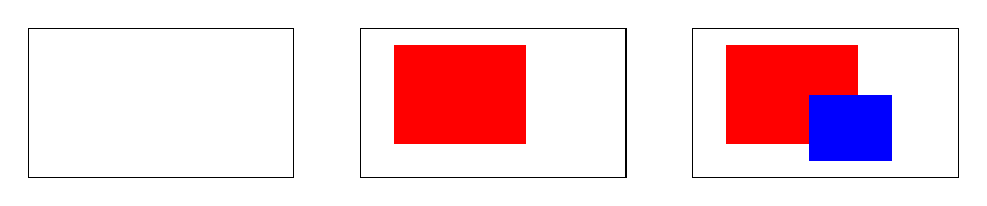
\begin{tikzpicture}[scale=6, x=1, y=-1]
			\draw        ( 0, 0) rectangle +(16, 9);

			\draw        (20, 0) rectangle +(16, 9);
			\fill[red]   (22, 1) rectangle +( 8, 6);

			\draw        (40, 0) rectangle +(16, 9);
			\fill[red]   (42, 1) rectangle +( 8, 6);
			\fill[blue]  (47, 4) rectangle +( 5, 4);
		\end{tikzpicture}
	\end{center}

	Whereas we really want this:

	\begin{center}
		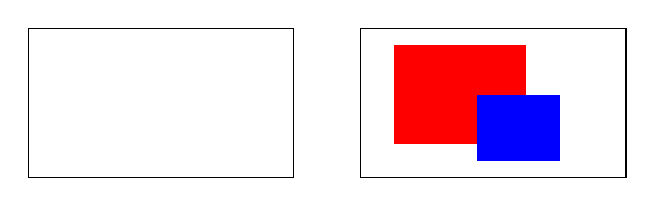
\begin{tikzpicture}[scale=6, x=1, y=-1]
			\draw        ( 0, 0) rectangle +(16, 9);

			\draw        (20, 0) rectangle +(16, 9);
			\fill[red]   (22, 1) rectangle +( 8, 6);
			\fill[blue]  (27, 4) rectangle +( 5, 4);
		\end{tikzpicture}
	\end{center}
\end{frame}

\begin{frame}
	\frametitle{Atomic Mode-Setting}
	\begin{itemize}
		\item allows an output configuration to be validated before it
			is applied:
			\begin{itemize}
				\item no hardware is touched before the driver acknowledges
					that the configuration is valid and can be applied
				\item no need for rollback
			\end{itemize}
		\item allows atomic updates of an output configuration:
			\begin{itemize}
				\item multiple planes updated at the same time
				\item perfect frames
			\end{itemize}
		\item allows for unification and simplification of drivers
			\begin{itemize}
				\item legacy code can be removed from drivers
				\item much of the handling moves into helpers
			\end{itemize}
	\end{itemize}
\end{frame}

\subsection{Building Blocks}

\begin{frame}
	\frametitle{Atomic Mode-Setting - Building Blocks}
	\begin{itemize}
		\item Universal Planes
		\item Properties
		\item Atomic State
	\end{itemize}
\end{frame}

\begin{frame}
	\frametitle{Universal Planes}
	\begin{itemize}
		\item root window is special in legacy KMS
			\begin{itemize}
				\item becomes a regular plane
				\item hardware treats them the same anyway
					\begin{itemize}
						\item code becomes simpler
					\end{itemize}
			\end{itemize}
		\item cursor exposed as plane
			\begin{itemize}
				\item exports a list of supported formats
			\end{itemize}
		\item helpers are available
			\begin{itemize}
				\item implement legacy IOCTLs using universal planes
				\item implement primary plane using legacy callbacks
			\end{itemize}
	\end{itemize}
\end{frame}

\begin{frame}
	\frametitle{Properties and Atomic State}
	\begin{itemize}
		\item interface parameters are converted to object properties
		\item properties are stored in atomic state objects
			\begin{itemize}
				\item blob properties are read-only, no way to change the
					video mode from userspace
			\end{itemize}
		\item atomic state objects are validated and applied
	\end{itemize}
\end{frame}

\section{Driver Conversion}

\subsection{Preparatory Work}

\begin{frame}
	\frametitle{Universal Planes}
	\begin{itemize}
		\item relatively easy to implement, matches what modern hardware
			exposes
		\item many drivers are already converted and can be used as a
			reference
	\end{itemize}
\end{frame}

\begin{frame}
	\frametitle{VBLANK Handling}
	\begin{itemize}
		\item atomic mode-setting has somewhat strict requirements
			\begin{itemize}
				\item plane updates are synchronized to VBLANKs to make sure
					framebuffers are unused before unreferenced
				\item good news because drivers don't have to worry anymore
			\end{itemize}
		\item drivers must disable VBLANK machinery when the display
			controller is off ({\tt drm\_crtc\_vblank\_off()})
		\item when the display controller is enabled the VBLANK machinery must
			be turned on again ({\tt drm\_crtc\_vblank\_on()})
	\end{itemize}
	Helpers fall over if the hardware state isn't accurately mirrored in the
	VBLANK machinery.
\end{frame}

\begin{frame}
	\frametitle{Driver Rewrite}
	\begin{itemize}
		\item atomic mode-setting has fairly high expectations
		\item especially important for atomic DPMS
		\item {\tt ->prepare()} is called when the CRTC or encoder is disabled
		\item {\tt ->mode\_set()} is called when the mode changes
		\item {\tt ->commit()} is used when the CRTC or encoder is enabled
	\end{itemize}
	On Tegra everything was done in {\tt ->dpms()}, requiring an almost
	complete rewrite.
\end{frame}

\subsection{Three Phases}

\begin{frame}
	\frametitle{Conversion in Three Phases}
	\begin{itemize}
		\item Phase 1 - Transitional Helpers
		\item Phase 2 - Atomic State Object Scaffolding
		\item Phase 3 - Rolling out Atomic Support
	\end{itemize}
	Transitional and atomic helpers are very modular and the conversion is
	suprisingly painless.
\end{frame}

\begin{frame}
	\frametitle{Phase 1 - Transitional Helpers}
	\begin{itemize}
		\item implement legacy entry points in terms of new atomic callbacks
			\begin{itemize}
				\item CRTCs
					\begin{itemize}
						\item {\tt ->atomic\_check()} - validate state
						\item {\tt ->atomic\_begin()} - prepare for updates
						\item {\tt ->atomic\_flush()} - apply updates atomically
						\item {\tt ->mode\_set\_nofb()} - apply CRTC timings
					\end{itemize}
					It is possible to set a mode without a primary plane.
				\item planes
					\begin{itemize}
						\item {\tt ->prepare\_fb()} - e.g. pin backing storage
						\item {\tt ->cleanup\_fb()} - e.g. unpin backing storage
						\item {\tt ->atomic\_check()} - validate state
						\item {\tt ->atomic\_update()} - plane updates
						\item {\tt ->atomic\_disable()} - disable plane
					\end{itemize}
			\end{itemize}
		\item caveat: {\tt ->atomic\_destroy\_state()} needs to be wired up
			here, otherwise the transitional helpers will leak state objects
	\end{itemize}
\end{frame}

\begin{frame}
	\frametitle{Phase 2 - Atomic State Object Scaffolding}
	\begin{itemize}
		\item wire up state callbacks for planes, CRTCs and connectors:
			\begin{itemize}
				\item {\tt ->reset()}
					\begin{itemize}
						\item {\tt drm\_atomic\_helper\_*\_reset()}
					\end{itemize}
				\item {\tt ->atomic\_duplicate\_state()}
					\begin{itemize}
						\item {\tt drm\_atomic\_helper\_*\_duplicate\_state()}
					\end{itemize}
				\item {\tt ->atomic\_destroy\_state()}
					\begin{itemize}
						\item {\tt drm\_atomic\_helper\_*\_destroy\_state()}
					\end{itemize}
			\end{itemize}
		\item default helpers are good enough for starters
	\end{itemize}
\end{frame}

\begin{frame}
	\frametitle{Phase 3 - Rolling out Atomic Support}
	\begin{itemize}
		\item Step 1 - switch to atomic helpers internally:
			\begin{itemize}
				\item Planes:
					\begin{itemize}
						\item {\tt drm\_atomic\_helper\_update\_plane()}
						\item {\tt drm\_atomic\_helper\_disable\_plane()}
					\end{itemize}
				\item Driver:
					\begin{itemize}
						\item {\tt drm\_atomic\_helper\_check()}
						\item {\tt drm\_atomic\_helper\_commit()}
					\end{itemize}
			\end{itemize}
			Driver now uses only atomic interfaces internally.
	\end{itemize}
\end{frame}

\begin{frame}
	\frametitle{Phase 3 - Rolling out Atomic Support}
	\begin{itemize}
		\item Step 2 - switch to atomic helpers for userspace IOCTLs:
			\begin{itemize}
				\item {\tt drm\_atomic\_helper\_set\_config()}
					\begin{itemize}
						\item {\tt DRM\_MODE\_IOCTL\_SET\_CRTC}
					\end{itemize}
				\item provide a custom {\tt ->atomic\_commit()} implementation
					\begin{itemize}
						\item to support asynchronous commits, required for
							page-flipping
					\end{itemize}
				\item {\tt drm\_atomic\_helper\_page\_flip()}
					\begin{itemize}
						\item {\tt DRM\_MODE\_IOCTL\_PAGEFLIP}
					\end{itemize}
			\end{itemize}

			Driver is now fully atomic (semantically).
	\end{itemize}
\end{frame}

\subsection{Follow-up Work}

\begin{frame}
	\frametitle{Rip out Cruft}
	\begin{itemize}
		\item {\tt ->mode\_set()} and {\tt ->mode\_set\_base()} are no longer
			used
			\begin{itemize}
				\item {\tt ->mode\_set\_nofb()} does what is necessary to set
					a mode
			\end{itemize}

		\item atomic DPMS
			\begin{itemize}
				\item DPMS standby and suspend are no more (w00t)
				\item {\tt ->disable()} and {\tt ->enable()} callbacks
				\item atomic DPMS is a full off or on cycle
			\end{itemize}
			Isn't this exactly what Tegra used to do before the almost
			complete rewrite? Almost, except the atomic helpers now keep
			track of everything.
	\end{itemize}
\end{frame}

\begin{frame}
	\frametitle{Where the fun begins}
	\begin{itemize}
		\item Subclassing atomic state:
			\begin{itemize}
				\item embed {\tt struct drm\_*\_state} in device-specific
					structures
				\item move device-specific data into these structures
			\end{itemize}
			Allows {\tt ->atomic\_check()} to cache information already
			computed. Simplifies other code because it doesn't need to
			recompute.
			% TODO Tegra conversion report
		\item Implement truly atomic updates:
			\begin{itemize}
				\item e.g. {\tt ->atomic\_flush()}
				\item "GO" bits
			\end{itemize}
			% TODO Tegra conversion report
	\end{itemize}
\end{frame}

\section{Future Work}

\subsection{Userspace}

\begin{frame}
	\frametitle{Userspace IOCTL}
	\begin{itemize}
		\item brand new in Linux v3.20
		\item still hidden behind drm.atomic parameter
		\item amalgamation of objects and properties:
			\begin{itemize}
				\item array of object IDs
				\item array of per-object property counts
				\item array of properties
				\item flags
					\begin{itemize}
						\item page-flip
						\item test-only
						\item non-block
						\item allow modeset
					\end{itemize}
			\end{itemize}
	\end{itemize}
\end{frame}

\subsection{Drivers}

\begin{frame}
	\frametitle{More cool stuff}
	\begin{itemize}
		\item hardware readout:
			\begin{itemize}
				\item {\tt ->reset()} reads state of hardware at driver load
					time
				\item no transition if no state is changed
				\item seamless transition between firmware or bootloader and
					kernel
			\end{itemize}
		\item unify asynchronous commits
			\begin{itemize}
				\item possibly via generic helpers
			\end{itemize}
		\item asynchronous page-flips
			\begin{itemize}
				\item {\tt eglSwapInterval()}
				\item because everybody loves benchmarks
				\item generic flip-queue that works for all drivers
					\begin{itemize}
						\item can fast-forward over a bunch of updates if
							supported by the driver
						\item it's like benchmarking page-flips, but without
							the tearing
					\end{itemize}
			\end{itemize}
		\item plane rotation via standard properties
	\end{itemize}
\end{frame}

\section{Summary}

\begin{frame}
	\frametitle{Summary}
	\begin{itemize}
		\item Atomic mode-setting is not only necessary but allows a bunch of
			nice and long overdue cleanup and unification.
		\item Atomic mode-setting is nowhere near as complicated as it sounds.
		\item Before converting your driver, make sure to have well-behaved
			callbacks and VBLANK handling.
		\item Given that the conversion is almost trivial because of excellent
			helpers.
		\item If you maintain a KMS driver, go convert it now, otherwise you
			are going to miss out on all the good stuff coming up.
	\end{itemize}
\end{frame}

\end{document}

% vim: sts=4 sw=4 ts=4
